\documentclass{beamer}

\usepackage{../cppenv}
\usepackage{../recdefs}

\usetheme{Rochester}
\usecolortheme{crane}

\usepackage{pifont}
\newcommand{\cmark}{\ding{51}}
\newcommand{\done}{\rlap{\(\square\)}{\raisebox{2pt}{\large\hspace{1pt}\cmark}}\hspace{-2.5pt}}

\title{CS100 Recitation 11}
\author{GKxx}
\date{May 2, 2022}

\AtBeginSubsection{
    \begin{frame}{Contents}
        \tableofcontents[currentsection, currentsubsection]
    \end{frame}
}

\begin{document}

\begin{frame}
    \maketitle
\end{frame}

\begin{frame}{Contents}
    \tableofcontents
\end{frame}

\section{Overview: A Federation of Languages}

\section{Overview: A Federation of Languages}

\begin{frame}{What have we learnt?}
    \begin{center}
        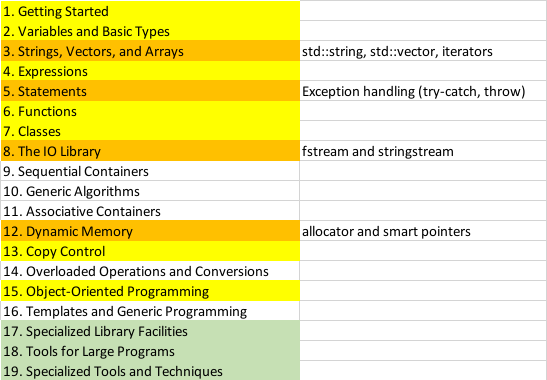
\includegraphics[width=0.95\textwidth]{img/contents.png}
    \end{center}
\end{frame}

\begin{frame}{A Federation of 4 Languages}
    \textit{Effective C++} Item 1: View C++ as a federation of languages.
    \begin{itemize}
        \item[\done] C
        \item[\done] Object-Oriented C++
        \item[\(\square\)] Template C++
        \item[\(\square\)] The STL
    \end{itemize}
\end{frame}

\section{Operator Overloading: First Glance}

\section{Operator Overloading: First Glance}

\begin{frame}{Operator Overloading}
    \begin{itemize}
        \item At least one class-type parameter.
        \item Cannot change the \textbf{precedence} or the \textbf{associativity}.
    \end{itemize}
    Operators that may be overloaded:
    \begin{center}
        \begin{tabular}{|cccccc|}
            \hline
            \ttt{+} & \ttt{-} & \ttt{*} & \ttt{/} & \ttt{\%} & \ttt{\^{}}\\
            \ttt{\&} & \ttt{|} & \ttt{\~} & \ttt{!} & \redtt{,} & \ttt{=}\\
            \ttt{<} & \ttt{>} & \ttt{<=} & \ttt{>=} & \ttt{++} & \ttt{--}\\
            \ttt{<<} & \ttt{>>} & \ttt{==} & \ttt{!=} & \redtt{\&\&} & \redtt{||}\\
            \ttt{+=} & \ttt{-=} & \ttt{/=} & \ttt{\%=} & \ttt{\^{}=} & \ttt{\&=}\\
            \ttt{|=} & \ttt{*=} & \ttt{<<=} & \ttt{>>=} & \ttt{[]} & \ttt{()}\\
            \ttt{->} & \ttt{->*} & \ttt{new} & \ttt{new[]} & \ttt{delete} & \ttt{delete[]}\\
            \hline
        \end{tabular}
    \end{center}
\end{frame}

\begin{frame}{Operator Overloading}
    Operators that may not be overloaded:
    \begin{center}
        \begin{tabular}{|cccc|}
            \hline
            \ttt{::} & \ttt{.} & \ttt{.*} & \ttt{?:}\\
            \hline
        \end{tabular}
    \end{center}
    Overloaded operator is a function:
    \begin{itemize}
        \item A special name: the \bluett{operator} keyword followed by the symbol of the operator.
        \item Non-member function: Operands are the parameters from left to right.
        \item Member function: The leftmost operand is implicitly bound to \bluett{this}. Other operands are the parameters from left to right.
    \end{itemize}
    \pause
    \textit{More Effective C++} Item 7 says that \blue{never overload operator \ttt{\&\&}, \ttt{||} and \ttt{,}}. Why?
\end{frame}

\begin{frame}{Operator Overloading}
    We have seen that
    \begin{itemize}
        \item The IO library overloads \bluett{operator<<} and \bluett{operator>>}.
        \item The string library overloads \bluett{operator+} and \bluett{operator[]}.
        \begin{itemize}
            \item Why won't `\ttt{"ABC" + "DEF"}' compile?
        \end{itemize}
    \end{itemize}
\end{frame}

\section{The IO Library}

\section{The IO Library}

\subsection{\ttt{<iostream>}}

\begin{frame}[fragile]{\ttt{iostream}, \ttt{cin} and \ttt{cout}}
    \begin{itemize}
        \item \ttt{std::cin}: object of type \ttt{std::istream}.
        \item \ttt{std::cout}: object of type \ttt{std::ostream}.
        \item \ttt{std::istream} and \ttt{std::ostream} are \textbf{uncopyable} types.
        \pause
        \item Outputs can be chained together as in `\ttt{cout << a << b}'. Why?
    \end{itemize}
    \pause
    \begin{cpp}
inline std::ostream &operator<<
        (std::ostream &os, const Point2d &p) {
  os << "(" << p.get_x() << ", " << p.get_y() << ")";
  return os;
}
    \end{cpp}
\end{frame}

\begin{frame}[fragile]{Test the State of \ttt{iostream}}
    On input failure, no error would be thrown, but we can test this by using the stream object as a condition.
    \begin{cpp}
struct Vector2d {
  double x, y, norm_l2;
};
inline std::istream &operator>>
        (std::istream &is, Vector2d &v) {
  is >> v.x >> v.y;
  // On input failure, set the object to a valid state.
  if (is)
    v.norm_l2 = std::sqrt(v.x * v.x + v.y * v.y);
  else
    v = Vector2d{};
  return is;
}
    \end{cpp}
\end{frame}

\begin{frame}[fragile]{Examples}
    Read an unknown number of integers?
    \begin{cpp}
std::vector<int> v;
int x;
while (std::cin >> x)
  v.push_back(x);
    \end{cpp}
    \pause
    Read a line as a string?
    \begin{cpp}
std::string line;
std::getline(std::cin, line);
    \end{cpp}
    \pause
    \begin{itemize}
        \item \ttt{std::getline} reads until the first newline character (`\textbackslash n'), and throws away that newline character.
        \item What happens?
        \begin{cpp}
int n; std::cin >> n;
std::string line;
std::getline(std::cin, line);
        \end{cpp}
    \end{itemize}
\end{frame}

\begin{frame}[fragile]{Manipulators}
    \ttt{endl}, \ttt{flush} and the like are \textbf{manipulators}.
    \begin{itemize}
        \item \ttt{endl} outputs a newline character and flushes the buffer.
        \item \ttt{flush} only flushes the buffer.
    \end{itemize}
    More manipulators: (some defined in \ttt{<iomanip>})
    \begin{itemize}
        \item \ttt{boolalpha}, \ttt{noboolalpha}
        \item \ttt{oct}, \ttt{hex}, \ttt{dec}, \ttt{showbase}, \ttt{noshowbase}, \ttt{setbase}
        \item \ttt{fixed}, \ttt{setprecision}, \ttt{scientific}
        \item \dots\dots
    \end{itemize}
    \textit{C++ Primer} 17.5
\end{frame}

\subsection{\ttt{<fstream>}}

\begin{frame}[fragile]{File Streams}
    Read an unknown number of integers from a file `\ttt{student\_score.txt}'?
    \begin{cpp}
std::ifstream infile("student_score.txt");
// Equivalent way:
// std::ifstream infile;
// infile.open("student_score.txt");
std::vector<int> score;
int x;
while (infile >> x)
  score.push_back(x);
infile.close();
    \end{cpp}
\end{frame}

\begin{frame}{Inheritance}
    \begin{columns}
        \begin{column}{0.6\textwidth}
            \begin{center}
                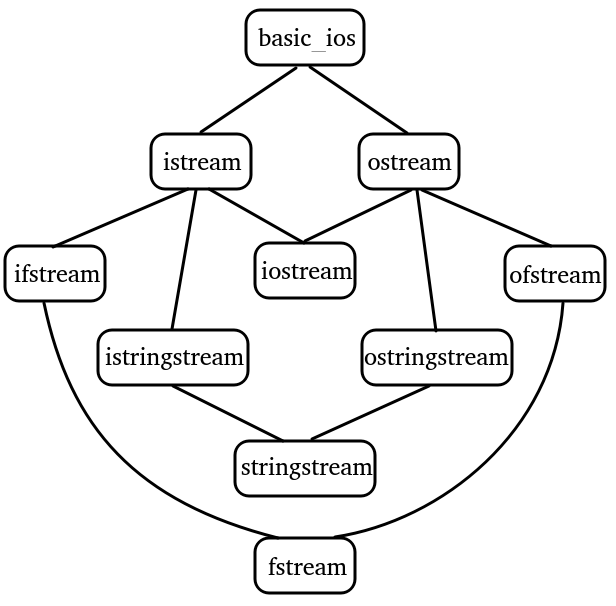
\includegraphics[scale=0.425]{img/iostream_inheritance.png}
            \end{center}
        \end{column}
        \begin{column}{0.4\textwidth}
            \begin{itemize}
                \item Multiple inheritance
                \item Virtual inheritance
                \item What can we know from this?
            \end{itemize}
        \end{column}
    \end{columns}
\end{frame}

\begin{frame}[fragile]{Real World Example}
    Read a `\ttt{.tex}' file. Change math from `\$\dots\$' to `\textbackslash(\dots\textbackslash)'.
    \begin{cpp}
std::ifstream infile("hw3.tex");
std::ofstream result("result.tex");
bool in_math = false;
std::string line;
while (std::getline(infile, line)) {
  // process the line
}
infile.close();
result.close();
    \end{cpp}
\end{frame}

\begin{frame}[fragile]{File Modes}
    Append something to a file, instead of overwriting it?
    \begin{cpp}
std::ofstream out_file("name.txt", std::ofstream::app);
    \end{cpp}
    \pause
    \begin{center}
        \begin{tabular}{|ll|}
            \hline
            \ttt{in} & Open for input\\
            \ttt{out} & Open for output\\
            \ttt{app} & Seek to the end before every write\\
            \ttt{ate} & Seek to the end immediately after the open\\
            \ttt{trunc} & Truncate the file\\
            \ttt{binary} & Do IO operations in binary mode\\
            \hline
        \end{tabular}
    \end{center}
    \begin{itemize}
        \item \textit{C++ Primer} 8.2.2
    \end{itemize}
\end{frame}

\subsection{\ttt{<sstream>}}

\begin{frame}[fragile]{Stringstreams}
    Read data from a string, or generate a string by writing different kinds of data.
    \begin{cpp}
struct Person_info {
  std::string name;
  std::vector<std::string> phones;
};
std::string line;
std::vector<Person_info> people;
while (std::getline(std::cin, line)) {
  Person_info info;
  std::istringstream record(line);
  record >> info.name;
  std::string phone;
  while (record >> phone)
    info.phones.push_back(phone);
  people.push_back(info);
}
    \end{cpp}
\end{frame}

\begin{frame}[fragile]{Stringstreams}
    Convert some \bluett{double} or \bluett{int} to a string?
    \begin{cpp}
inline std::string convert(double value) {
  std::ostringstream oss;
  oss << value;
  return oss.str();
}
    \end{cpp}
    \pause
    It works, but \ttt{std::to\_string} is a better choice!
\end{frame}

\section{Sequential Containers}

\subsection{Overview}

\begin{frame}{Sequential Containers}
    The standard library provides the following sequential containers:
    \begin{center}
        \begin{tabular}{|ll|}
            \hline
            \ttt{vector} & Flexible-size array.\\
            \ttt{deque} & Double-ended queue.\\
            \ttt{list} & Doubly-linked list.\\
            \ttt{forward\_list} & Singly-linked list.\\
            \ttt{array} & Encapsulation of built-in array.\\
            \ttt{string} & A specialized container containing characters.\\
            \hline
        \end{tabular}
    \end{center}
\end{frame}

\begin{frame}{Consistent Interfaces}
    \begin{figure}[h]
        \centering
        \begin{minipage}{0.48\textwidth}
            \centering
            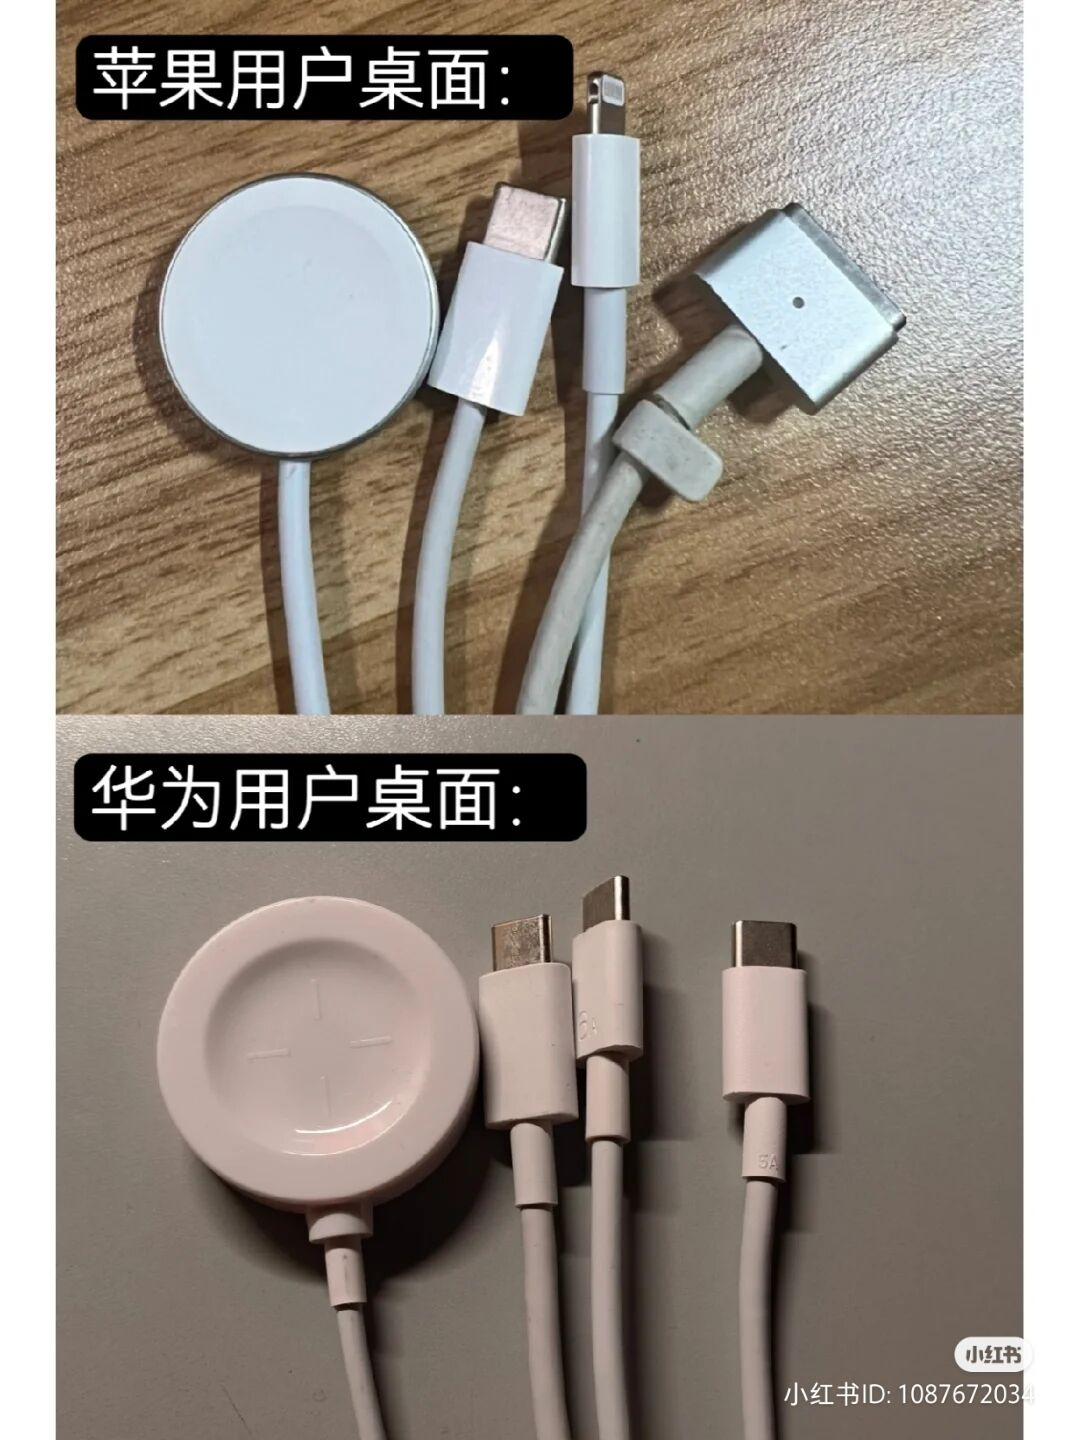
\includegraphics[scale=0.135]{figures/interface1.jpg}
        \end{minipage}
        \begin{minipage}{0.48\textwidth}
            \centering
            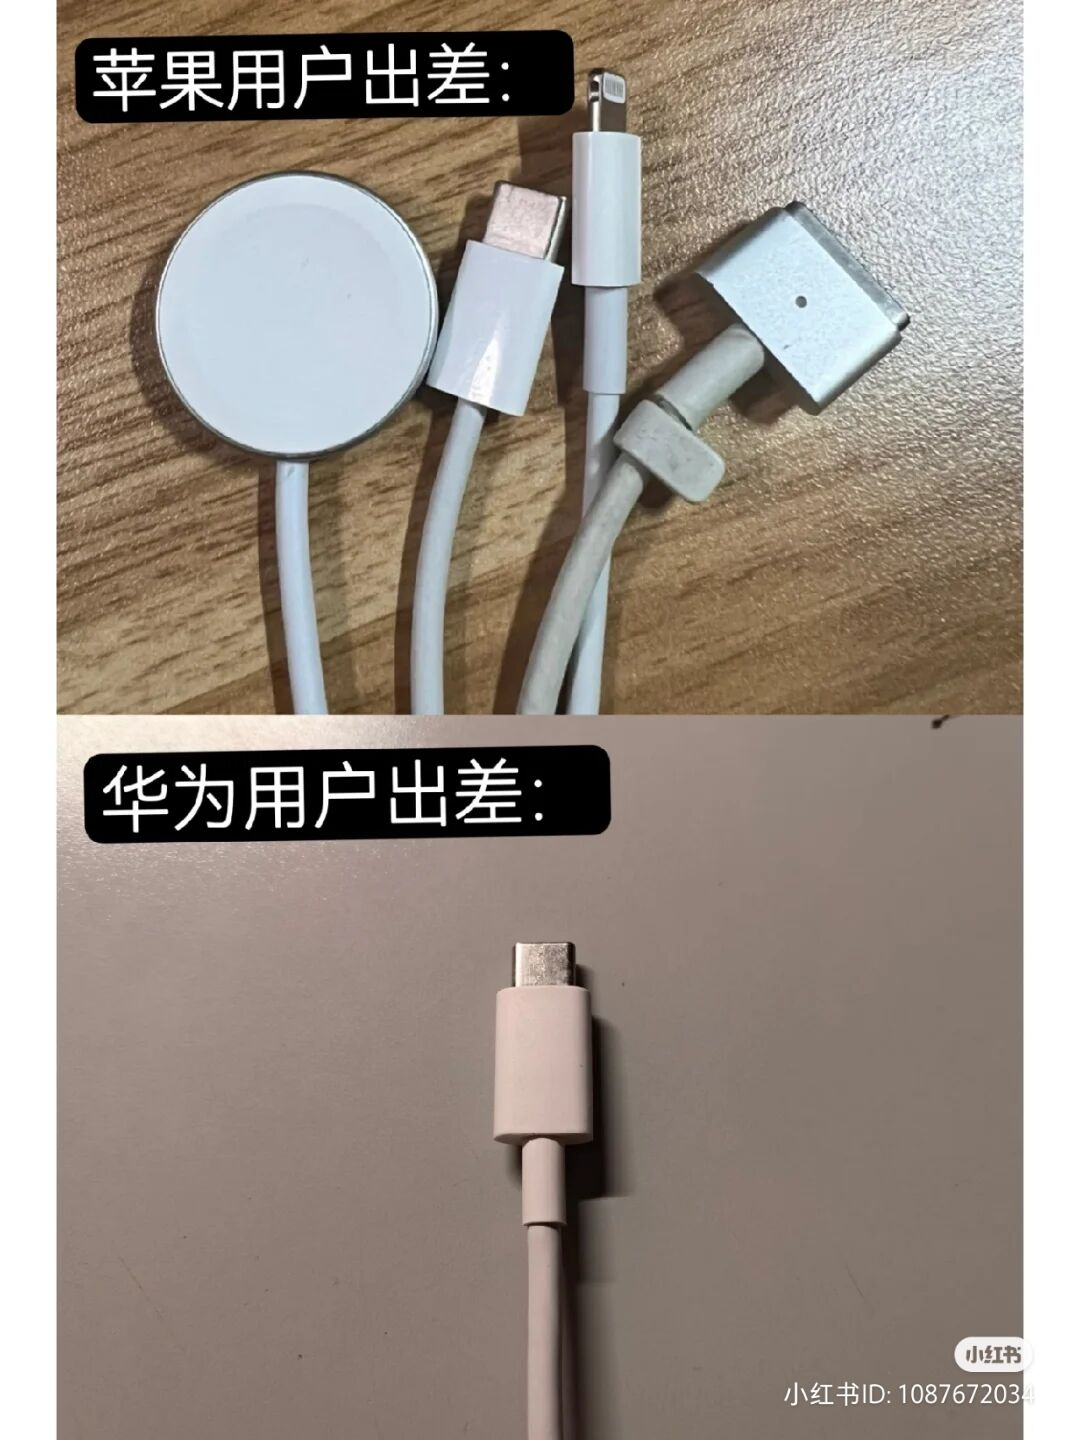
\includegraphics[scale=0.135]{figures/interface2.jpg}
        \end{minipage}
    \end{figure}
\end{frame}

\begin{frame}{Data }
\end{frame}

\end{document}